\Transcb{yellow}{blue}{The Neutrino-Gamma connection}
\onecolumn
\begin{center}
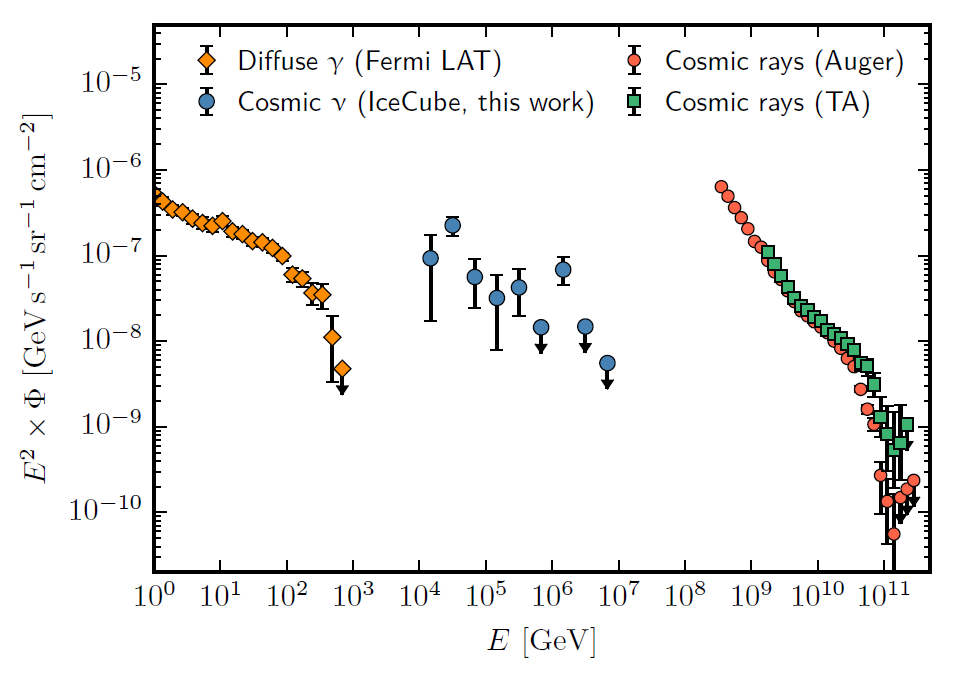
\includegraphics[keepaspectratio,height=12cm]{Fermi-IC-CR}\\
{\large [Lars Mohrmann, PhD 2015, Humboldt University Berlin]}
\end{center}
%
{\blue
Common astrophysical sources ?\\
$N+\gamma \rightarrow \Delta \rightarrow \pi+{\red N \text{~(CR)}}
 \qquad \pi^{0} \rightarrow {\red \gamma\gamma \text{~(Fermi)}} \qquad \pi^{\pm} \rightarrow {\red \nu,\bar{\nu} \text{~(IceCube)}}$
}

\Tr
\onecolumn
\begin{center}
{\blue Follow up for transients on neutrino alerts}
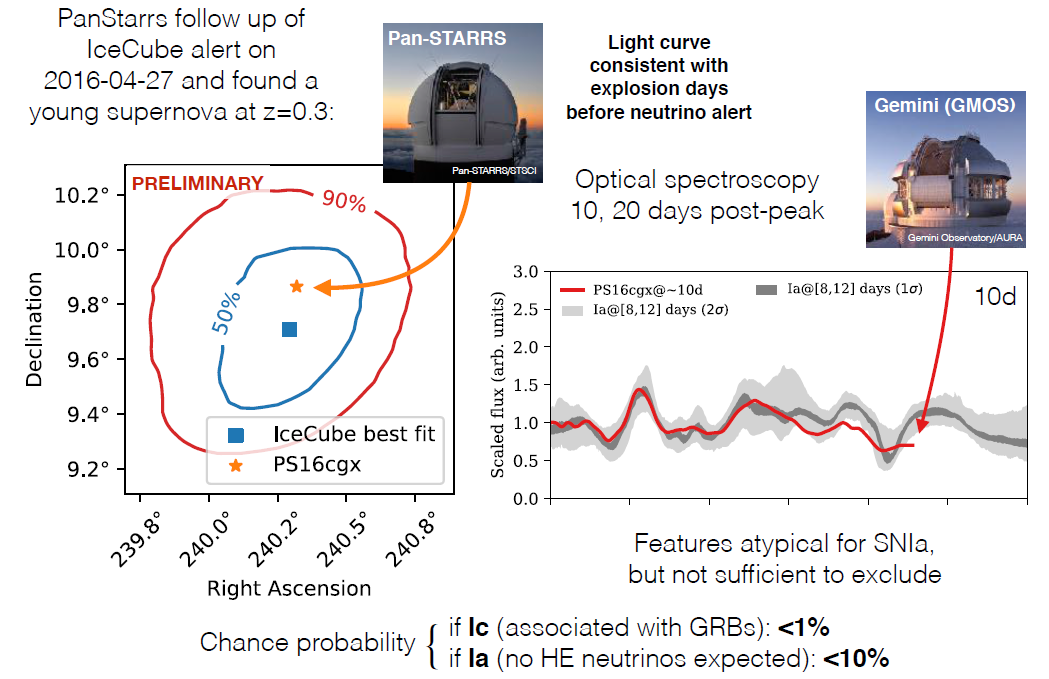
\includegraphics[keepaspectratio,height=14cm]{IC160427A}\\
{\large [Credit M. Kowalski SuGAR2018]}
\end{center}

\Tr
\onecolumn
\begin{center}
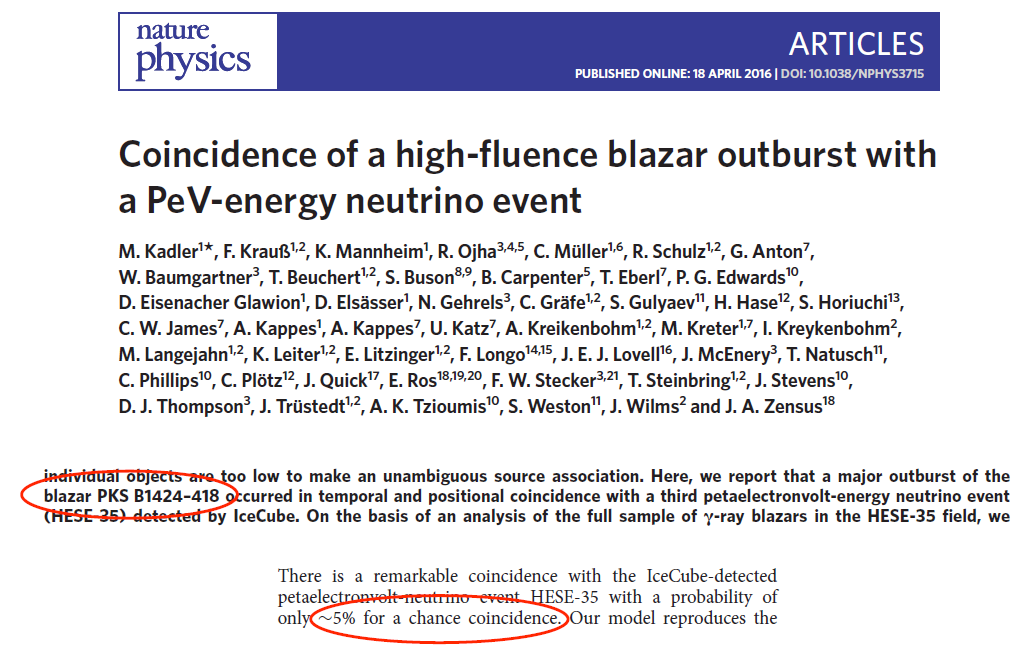
\includegraphics[keepaspectratio,height=14cm]{HESE35}\\
{\large [Credit M. Ahlers SuGAR2018]}
\end{center}

\Tr
\onecolumn
\vspace*{6cm}
\begin{center}
{\red \shabox{\Huge Multi-messenger studies look promising !}}
\end{center}

\Tr
{\blue IceCube: Track with $E_{dep} \sim 24$ TeV observed at 22-sep-2017 20:54:30.43 UTC}\\
$\rightarrow$ EHE alert (IC170922A) issued ($\sim 4$ per year) 
\begin{center}
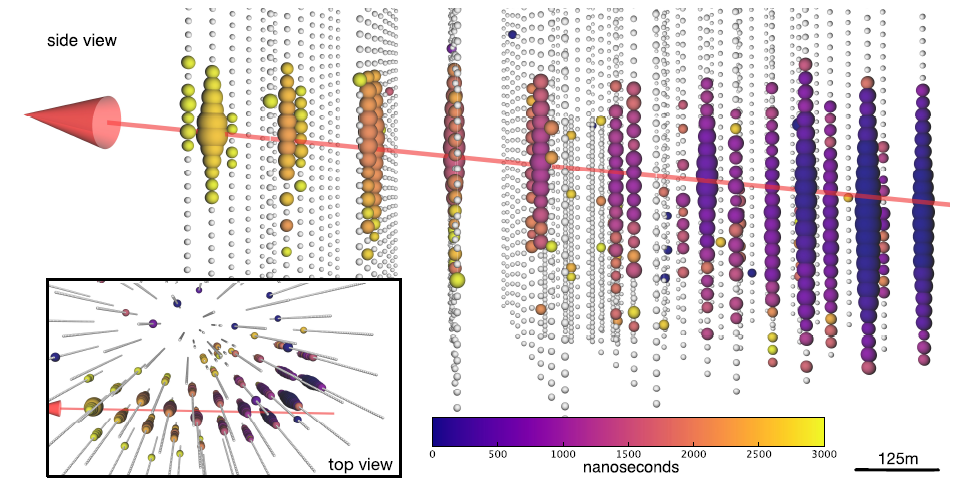
\includegraphics[keepaspectratio,height=12cm]{IC170922A-event}
\end{center}
IC170922A track parameters: $\alpha=77.4^{\circ} \quad \delta=5.7^{\circ} \quad E_{\nu}=290$ TeV
